\section{Meccanica Newtoniana}


\subsection{L'equazione di Newton}
\begin{equation}
    f = m a 
\end{equation}
Il \textit{secondo principio della dinamica} di Newton è l'equazione del moto di una particella di massa $m$ 
soggetta a una forza $f$, $a$ è l'accelerazione.\\ 
\begin{equation}
    m \ddot{x} = f( x(t),\dot{x}(t), t) \qquad \text{ ove } \quad v = \dot{x}(t) = \dv{x}{t}\quad a = \ddot{x}(t)= \dv[2]{x}{t}
\end{equation}

La forza $f$ è una funzione assegnata del tipo $f: \mathbb{R}^d\times \mathbb{R}^d \times \mathbb{R} \rightarrow \mathbb{R}^d$\\
L'equazione di newton è un'\textit{equazione differenziale ordinaria} ODE di secondo ordine con incognita $x(t)$. 
In base ai dati iniziali e alla funzione $f$ possono valere o meno i teoremi di esistenza e unicità $\exists!$ locale e globale.\\ 
$x(t)$ è una curva del tipo $I \subseteq \mathbb{R}\quad x: I \rightarrow \mathbb{R}^d $. L'equazione può essere 
riscritta nella forma di sistema equivalente:
\begin{equation}
    \begin{cases}
        \dot{x}(t) = v(t)\\ 
        \dot{v}(t) =\frac{1}{m} f( x(t), v(t), t)
    \end{cases}
    \implies
    \qquad
    \dot{X}(t)= F(t)
\end{equation}
ove:
\begin{equation*}
    X (t) = \begin{pmatrix}
        x (t) \\ 
        v (t)
    \end{pmatrix} \subseteq \mathbb{R}^d \times \mathbb{R}^d \simeq \mathbb{R}^{2d} \qquad
    F (t) = \begin{pmatrix}
        v(t) \\
        f(x(t), v(t),t)
    \end{pmatrix}
\end{equation*}

Il moto può essere univocamente determinato se assegno il dato iniziale $x(t_0)=x_0,\;\dot{x}(t_0)= v(t_0)=v_0$.\\
Conoscendo i dati iniziali, cerchiamo una soluzione locale tramite sviluppo di Taylor: 
\begin{equation*}
    x(t_0) \text{ noto}\implies x(t_0+h)= x(t_0)+\dot{x}(t_0) h +\frac{1}{2!}\ddot{x}(t_0) h^2 +\frac{1}{3!}\dddot{x}(t_0)h^3  + o(h^4)= 
\end{equation*}
\begin{equation*}
   = x_0 +v_0 h + \frac{f}{2m}(x_0,v_0,t_0) h^2 + \dots
\end{equation*}

Si può scrivere:
\begin{equation}
    \begin{cases}
        \dd{x}= v(t)\dd{t}\\
        \dd{v}= \frac{1}{m}f(x(t),v(t),t)\dd{t} 
    \end{cases}
\end{equation}
\begin{equation*}
    (x,v) \text{ in } t \implies  \text{ in } t +\dd{t} \quad (x',v')= (x+\dd{x},v+\dd{v})= (x+v\dd{t},v+ \frac{f}{m}\dd{t})
\end{equation*}

\begin{definition}
    \begin{equation*}
        \begin{pmatrix}
            x\\v  
        \end{pmatrix}\in \mathbb{R}^{2d} 
    \end{equation*}
    è detto \textit{spazio delle fasi} del sistema. 
\end{definition}

\begin{definition}
    La curva soluzione $t\rightarrow(x(t),v(t))$ si chiama \textit{curva di fase}, distinta da $t\rightarrow x(t)$ che si chiama 
    \textit{traiettoria o orbita}.
\end{definition}

\begin{definition}
    \begin{equation*}
        F=\begin{pmatrix}
            v\\\frac{1}{m}f 
        \end{pmatrix}
    \end{equation*}
    si chiama \textit{campo vettoriale newtoniano} ed è geometricamente il vettore tangente alla curva di fase passante per $(x,v)$ al tempo $t$.
\end{definition}

\begin{definition}
    La soluzione del sistema newtoniano corrispondente dal dato iniziale $(x_0, v_0)$ in $\mathbb{R}^{2d}$ si indica con 
    $\Phi_N^t(x_0,v_0)$ e si chiama \textit{flusso del campo vettoriale newtoniano}
    \begin{equation}
        \Phi_N^t; \mathbb{R}^{2d}\rightarrow\mathbb{R}^{2d} ; \qquad \Phi_N^0 (x_0,v_0)= (x_0,v_0) 
    \end{equation}
\end{definition}

%esercizio 1  iterativo

% Reazione di radiazione di Lorentz



\subsection{Modelli di forza}

\subsubsection{Spazialmente uniformi}
In cui la forza non dipende dalla posizione: $f = f(v,t)$.
\begin{example}
    $f = -\gamma v $ Attrito viscoso
\end{example}
\begin{example}
    $f = q(E_0+ \frac{v}{c}\times B_0)$ Forza di Lorents in campi uniformi
\end{example}



\subsubsection{Puramente posizionali}
Forze indipendenti dalla velocità: $f= f(x,t)$. Distinguiamo inoltre le \textit{forze potenziali} in cui esiste un potenziale scalare $U(x,t)$
tale che:
\begin{equation}
    f= -\nabla_xU(x,t)= -\pdv{U}{x}(x,t)
\end{equation}

Le forze potenziali indipendenti dal tempo sono dette \textit{forze conservative}.
\begin{theorem}
    Per un sistema newtoniano conservativo, la funzione energia totale
    \begin{equation}
        H(x,\dot{x}):= K +U := \frac{1}{2}m\abs{\dot{x}}^2+U(x)
    \end{equation}
    è costante lungo le soluzioni della equazione del moto.
\end{theorem}
\begin{proof}
    Per una forza conservativa: $m\ddot{x}= -\nabla_xU(x)$
    \begin{equation*}
        \implies \dot{x}\cdot (m\ddot{x})= -\dot{x} \cdot\nabla_xU \implies m\dv{}{t}\left( \frac{\abs{\dot{x}}^2}{2} \right)= -\dv{}{t}U(x(t))
    \end{equation*}
    \begin{equation}
        \implies \dv{}{t}\left( \frac{m\abs{\dot{x}}^2}{2} +U(x) \right) = 0
    \end{equation}
\end{proof}

Il moto avviene nell'insieme di livello $H^{-1}(E)$ dove $E = H(x_0,v_0)$, detta \textit{superficie equipotenziale}.
\begin{equation}
    \Sigma_E:= H^{-1}(E)=\left\{ (x,v) \in \mathbb{R}^{2d}:H(x,v)=E  \right\} 
\end{equation}

\begin{proposition}
    Il moto è sempre tangente alla supericie equipotenziale.
\end{proposition}
\begin{proof}
    \begin{equation*}
        H(x,v)= m\frac{\abs{v}^2}{2}+U(x) \implies 
        \nabla H(x,v)= 
        \begin{pmatrix}
            \nabla_xU\\mv 
        \end{pmatrix}
        \qquad \dot{X}= 
        \begin{pmatrix}
            v\\\frac{f}{m}
        \end{pmatrix}
    \end{equation*}
    \begin{equation*}
        \nabla H \cdot \dot{X}=  
        \begin{pmatrix}
            \nabla_xU\\mv 
        \end{pmatrix} \cdot
        \begin{pmatrix}
            v\\\frac{f}{m}
        \end{pmatrix}
        = v\cdot\nabla_xU +v\cdot f = -v \cdot f +v\cdot f = 0 
    \end{equation*}
\end{proof}

\begin{remark}
    $\Sigma_E $ ha dimensione $2d-1$
\end{remark}

Suppongo di avere una forza genererica per cui $m\ddot{x}= f $, cerchiamo U(x) tale che $H(x,v)$ si conservi lungo i moti.
\begin{equation*}
    \dv{}{t}H(x(t),v(t))= \nabla_xH\cdot\dot{x}+\nabla_v\cdot\dot{v}= \nabla_xU\cdot + mv\cdot \frac{f}{m}\equiv0
\end{equation*}
\begin{equation}
    \implies v \cdot \left( f + \nabla_xU \right)=0
\end{equation}
Questo implica che possono esserci componenti della forza perpendicolari alla velocità dette \textit{giroscopiche}.
\begin{equation}
    f= -\nabla_xU + v\times (\dots)
\end{equation}



\subsubsection{Forze centrali}

\begin{definition}
    Una forza $f(x,v,t)$ si dice \textit{centrale} se è diretta come il vettore posizione $x$ a ogni istante, ossia:
    \begin{equation}
        f(x,v,t)= \Psi(x,v,t)x= \varphi(x,v,t)\hat{x}
    \end{equation}
    dove $\Psi,\varphi: \mathbb{R}^d\times \mathbb{R}^d \times \mathbb{R} \rightarrow \mathbb{R}$ e $\varphi=\Psi\abs{x}, \;\hat{x}=\frac{x}{\abs{x}}$.
\end{definition}

\begin{definition}
    L'origine, in un campo di forze centrali, si chiama \textit{centro della forza}. $\varphi$ è lo \textit{scalare della forza}.
\end{definition}

\begin{proposition}
    La quantità vettoriale $\ell(x,\dot{x}):= x\times m\dot{x}$, detta \textit{momento angolare}, si conserva lungo i moti newtoniani con forze centrali.
\end{proposition}
\begin{proof}
    \begin{equation*}
        m\ddot{x}= f= \varphi\hat{x};  \qquad \dv{\ell}{t}= \dv{t}\left( x(t)\times m\dot{x}(t)\right)= 
        \dot{x}(t)\times m\dot{x}(t)+ x(t)\times m\ddot{x}(t)=
    \end{equation*}
    \begin{equation}
        m(\dot{x}\times\dot{x})+x\times f= \varphi x \times \hat{x}=0
    \end{equation}
\end{proof}

\begin{proposition}
    Il moto della particella dunque si svolge sul piano ortogonale a $ell$ di equazione: $\ell\cdot x =0$
\end{proposition}
\begin{proof}
    Dimostro che il piano $\pi:\ell\cdot x=0$ è invariante:
    \begin{equation}
        \ell\cdot x= (x(t)\times m\dot{x}(t))\cdot x(t)=0 \qquad\forall \, t
    \end{equation}
\end{proof}

\begin{remark}
    Dunque i moti centrali sono piano e si può ridurre di una dimensione
\end{remark}
\begin{definition}
    La \textit{velocità areolare } è l'area spazzata dal raggio vettore $x(t)$ nell'unità di tempo.
\end{definition}

\begin{proposition}
    La velocità areolare nei moti centrali è costante. Questa è anche detta \textit{seconda legge di Keplero}.
\end{proposition}
\begin{proof}
    Considero la variazione di area $\Delta A$ spazzata dal raggio vettore $x(t)$ in un intervallo di tempo $\Delta t$:
    \begin{equation*}
        \Delta A \simeq \frac{1}{2} \abs{ x(t) \times (x(t+\Delta t) - x(t)) } = \frac{1}{2} \abs{ x(t) \times \dot{x}(t) } \Delta t
    \end{equation*}
    \begin{equation}
        \dot{A}(t) = \lim_{\Delta t \to 0} \frac{\Delta A}{\Delta t} = \frac{1}{2} \abs{ x(t) \times \dot{x}(t) }
    \end{equation}
    \begin{equation}
        \dot{A}(t) = \frac{1}{2m} \abs{ x(t) \times m\dot{x}(t) } = \frac{1}{2m} \abs{ \ell } \qquad \textit{Legge della vel. areolare}
    \end{equation}
    Poiché $\ell$ si conserva nei moti centrali, segue che $\dot{A}(t)$ è costante.
\end{proof}



\subsubsection{Forze centrali autonome, posizionali a simmetria sferica}
Forze in cui la forza dipende solamente dal modulo del vettore posizione:
\begin{equation}
    f:= \varphi(\abs{x})\hat{x}
\end{equation}

Se $x= Rx'$ dove $R$ è una matrice di rotazione:
\begin{equation}
    \abs{x}= \abs{Rx'}= \sqrt{(Rx')\cdot(Rx')}= \sqrt{x'\cdot(R^\intercal R)x'}= \abs{x'}
\end{equation}
\begin{equation}
    \hat{x}=\frac{x}{\abs{x}}= \frac{Rx'}{\abs{Rx'}}= \frac{Rx'}{\abs{x'}}=R\hat{x}'
\end{equation}

\begin{proposition}
    $f= \varphi(\abs{x})\hat{x}$ è conservativa.    
\end{proposition}
\begin{proof}
    Consideriamo un potenziale:
    \begin{equation}
        U(\abs{x}):=-\int^\abs{x}\varphi(r)\dd{r}
    \end{equation}
    \begin{equation*}
        -\nabla_x U(\abs{x}) = -U'(\abs{x}) \nabla_x (\abs{x}) = -U'(\abs{x}) \nabla_x (\sqrt{x \cdot x}) 
    \end{equation*}
    \begin{equation*}
        = -U'(\abs{x}) \frac{\nabla_x (x \cdot x)}{2 \sqrt{x \cdot x}} = -U'(\abs{x}) \frac{2x}{2 \abs{x}} = -U'(\abs{x}) \hat{x}
\end{equation*}
\end{proof}

\begin{remark}
    Si ricava che la forma più generale per cui una forza centrale $f= \varphi(x)\hat{x}$ sia conservativa è $\varphi(x)=\varphi(\abs{x})$.
\end{remark}
\begin{proof}
    Usando le coordinate polari sferiche:     ($r = \abs{x}$)
    \begin{equation}
        \begin{cases}
            x_1 = r \sin\theta \cos\phi \\
            x_2 = r \sin\theta \sin\phi \\
            x_3 = r \cos\theta 
        \end{cases}
    \end{equation}
    Calcoliamo le derivate parziali di $U$:
    \begin{equation*}
        \pdv{U}{\theta}= \pdv{U}{x_1}\pdv{x_1}{\theta}+\pdv{U}{x_2}\pdv{x_2}{\theta}+\pdv{U}{x_3}\pdv{x_3}{\theta}=
         \left( \nabla_xU \right)\cdot\pdv{x}{\theta}= -\frac{\varphi(x)}{\abs{x}}\frac{1}{2}\pdv{\theta}\left( x\cdot x \right)
    \end{equation*}
    \begin{equation}
        =-\varphi(x)\frac{1}{\abs{x}}x\cdot \pdv{x}{\theta}= - \varphi(x)\frac{1}{2\abs{x}}\pdv{\theta}\abs{x}^2
        =- \varphi(x)\frac{1}{2\abs{x}}\pdv{r^2}{\theta}\equiv0 
    \end{equation}
    Perché $r$ e $\theta$ sono linearmente indpendenti.\\
    Analogamente si dimostra che $\pdv{U}{\phi}=0$.
    \begin{equation*}
        U = U(r) = U(\abs{x})\implies \nabla_xU= U'(\abs{x})\hat{x}
    \end{equation*}
    \begin{equation*}
        \varphi(x)\hat{x}=-U'(\abs{x})\hat{x}\implies \varphi(x)= -U'(\abs{x})
    \end{equation*}
\end{proof}

Le forza fondamentali di questo tipo sono la \textit{forza gravitazionale} e la \textit{forza elettrostatica} 
con rispettivamente la \textit{legge di Hooke-Newton} e la \textit{legge di Coulomb}:
\begin{equation}
    \varphi_G(\abs{x})= -G\frac{Mm}{\abs{x}^2}\qquad \quad \varphi_{es}(\abs{x})=\frac{Qq}{\abs{x}^2}
\end{equation}

Un'altra forza importante è la \textit{forza elastica}, descritta dalla \textit{legge di Hooke}:
\begin{equation}
    \varphi_{el}(\abs{x})= -k\abs{x}
\end{equation}

%Accenno di Lagrange e Hamilton


\subsection{Problemi}


\subsubsection{Oscillatore armonico tridimensionale}
\begin{equation}
    m\ddot{x}= f \qquad f = \varphi(\abs{x})\hat{x}\qquad \varphi = -kr
\end{equation}
E' una forza centrale: $\ell= x\times m\dot{x}$ è costante.\\
E' uno dei tipi di forze che produce orbite elittiche. 
E' stato candidato per la forza gravitazionale, ma la forza non è centrata nei fuochi
e il periodo non dipende dall'ampiezza.\\

Per $\ell  \neq 0$, cambio le coordinate a un sistema in cui:
\begin{equation}
    x_3 \parallel \ell; \quad x_1,x_2 \in x\cdot\ell=0  \qquad (3D\rightarrow 2D)
\end{equation}

Risolviamo l'equazione del moto:
\begin{equation*}
    m\ddot{x}= -kx \implies \ddot{x}= -\omega^2 x \text{ con } \omega= \sqrt{\frac{k}{m}}
\end{equation*}
In componenti:
\begin{equation}
    \begin{cases}
        \ddot{x}_1= -\omega^2 x_1\\
        \ddot{x}_2= -\omega^2 x_2
    \end{cases}\implies
    x_1 = a \cos(\omega t +\phi)\quad x_2= b\cos(\omega t + \psi)
\end{equation}
\begin{remark}
    Il periodo $T$ non dipende da $a$ e $b$:
    \begin{equation}
        T = \frac{2\pi}{\omega}= 2\pi\sqrt{\frac{m}{k}}
    \end{equation} 
\end{remark}

Definiamo: $\theta:=\omega t + \phi, \quad\delta:=\psi-\phi$.
\begin{equation}
    \implies \begin{cases}
        x_1 = a\cos(\theta)\\
        x_2 = b\cos(\theta+\delta)
    \end{cases}
\end{equation}

Se $\delta=0\implies x_1= a\cos(\theta),\;x_2=b\cos(\theta)\implies x_1=\frac{a}{b}x_2$ è il caso lineare in cui $\ell = 0$.
Se $\delta= \pi$ è uguale al caso precedente.\\
Se $\delta\neq 0$:
\begin{equation*}
    \begin{cases}
        x_1 = a\cos(\theta)\\
        x_2 = b(\cos(\theta)\cos(\delta)-\sin(\theta)\sin(\delta))
    \end{cases}
\end{equation*}
\begin{equation}
    \cos(\theta)=\frac{x_1}{a} \quad \frac{x_2}{b}= \frac{x_1}{a}\cos(\delta)-\sin(\theta)\sin(\delta)\implies
    \sin(\theta)= \frac{1}{\sin(\delta)}\left(  \frac{x_1}{a}\cos(\delta)-\frac{x_2}{b}\right)
\end{equation}

Applico l'ugualianza:
\begin{equation*}
    \frac{x_1^2}{a^2} + \frac{1}{\sin^2\delta}
      \left( \frac{x_1}{a}\cos\delta - \frac{x_2}{b} \right)^2= 1
\end{equation*}
\begin{equation*}
    \frac{x_1^2}{a^2} + \frac{1}{\sin^2\delta}
    \left( \frac{x_1^2}{a^2}\cos^2\delta - 2\frac{x_1 x_2}{a b}\cos\delta + \frac{x_2^2}{b^2} \right) = 1
\end{equation*}
\begin{equation}
    \left( 1 + \frac{\cos^2\delta}{\sin^2\delta} \right) \frac{x_1^2}{a^2}
    + \frac{1}{\sin^2\delta}\frac{x_2^2}{b^2}- 2\frac{\cos\delta}{\sin^2\delta}\frac{x_1 x_2}{a b} = 1
\end{equation}
Riscriviamola nella forma $x\cdot Mx = 1$:
\begin{equation}
    M = 
    \begin{pmatrix}
        \dfrac{1}{a^2 \sin^2 \delta} & -\dfrac{\cos \delta}{a b \sin^2 \delta} \\[1.2ex]
        -\dfrac{\cos \delta}{a b \sin^2 \delta} & \dfrac{1}{b^2 \sin^2 \delta}
    \end{pmatrix}
\end{equation}
$M$ è matrice simmetrica e reale, dunque si può applicare il teorema spettrale:
\begin{equation}
    \implies \exists\,R, \;R^\intercal R = 1 \quad t.c. \quad R^\intercal MR = \operatorname{diag} (m_1,m_2)
\end{equation}
Dove $m_1$ e $m_2$ sono gli autovalori reali di $M$. Esiste dunque un vettore $y:= R^\intercal x$ per cui:
\begin{equation}
    x\cdot Mx= (Ry)\cdot M(Ry)= y\cdot(R^\intercal MR)y= y\cdot \left( \operatorname{diag} (m_1,m_2) y\right)= m_1 y_1^2+m_2y_2^2=1
\end{equation}
Che è l'equazione per un elisse.
\begin{remark}
    Possiamo riscriverla come: $m_1 y_1^2+m_2y_2^2=\frac{y_1^2}{A^2}+\frac{y_2^2}{B^2}= 1$
\end{remark}
\begin{proof}
    \begin{equation*}
       \tr(M )>0, \det(M ) = \frac{1}{a^2b^2\sin[2](\delta)}>0\implies m_1+m_2>0, \quad m_1m_2>0 
    \end{equation*}
\end{proof}

\paragraph{RECAP Elisse}
La definizione geometetrica di un elisse è il luogo dei punti tale che $d_1+d_2= 2a$.
La definizione cartesiana è:
\begin{equation}
    \frac{x_1^2}{a^2}+ \frac{x_2^2}{b^2}=1 \quad \text{ con } a,b \in \mathbb{R}
\end{equation}
La definizione in coordinate polari:
\begin{equation}
    r = \frac{P}{1+\varepsilon\cos(\theta)} \quad \text{ con } P,\varepsilon \in \mathbb{R}
\end{equation}
Nella definizione in coordinate polari il centro è uno dei due fuochi, $\varepsilon \in [0,1)$ è detta eccentricità
e il parametro $P=r(\frac{\pi}{2})$.
Dimostriamo che queste tre definizioni siano equivalenti.
\begin{proof}
    1) $\leftrightarrow$ 2)\\
    Consideriamo le distanze di un punto generico $(x, y)$ dai due fuochi $F_1, F_2$. Sappiamo che:
    \begin{equation}
        \begin{cases}
            d_1^2 = (x - f)^2 + y^2 \\
            d_2^2 = (x + f)^2 + y^2
        \end{cases}
        \qquad
        (d_1 + d_2)^2 = 4a^2
    \end{equation}
    \begin{equation}
        d_1^2 + d_2^2 + 2 d_1 d_2 = 4a^2 \implies 4 d_1^2 d_2^2 = \left[ 4a^2 - (d_1^2 + d_2^2) \right]^2
    \end{equation}
    Sviluppando i conti si ottiene:
    \begin{equation}
        (a^2 - f^2)x^2 + a^2 y^2 = a^2(a^2 - f^2) \implies \frac{x^2}{a^2} + \frac{y^2}{a^2 - f^2} = 1
    \end{equation}

    2) $\leftrightarrow$ 3)\\
    Usando il cambio di coordinate polari:
    \begin{equation}
        \begin{cases}
            x = f + r \cos\theta \\
            y = r \sin\theta
        \end{cases}
    \end{equation}
    Sostituendo nell'equazione cartesiana:
    \begin{equation*}
        (a^2 - f^2)(f + r\cos\theta)^2 + a^2 r^2 \sin^2\theta = a^2(a^2 - f^2)
    \end{equation*}
    \begin{equation*}
        (a^2 - f^2)f^2 + 2f(a^2 - f^2)r\cos\theta + \left[(a^2 - f^2)\cos^2\theta + a^2\sin^2\theta\right] r^2 = a^2(a^2 - f^2)
    \end{equation*}
    \begin{equation*}
        \left[(a^2 - f^2)\cos^2\theta + a^2\sin^2\theta\right] r^2 + 2f(a^2 - f^2) r\cos\theta + (a^2 - f^2)f^2 - a^2(a^2 - f^2) = 0
    \end{equation*}
    \begin{equation}
        \left(a^2 - f^2\cos^2\theta\right) r^2 + 2f(a^2 - f^2) r\cos\theta - (a^2 - f^2)^2 = 0
    \end{equation}
    Risolvendo come equazione di secondo grado in $r$:
    \begin{equation*}
        r = \frac{-(a^2 - f^2)f\cos\theta + \sqrt{(a^2 - f^2)^2 a^2}}{a^2 - f^2\cos^2\theta}
    \end{equation*}
    Considerando solo la soluzione positiva:
    \begin{equation}
        r = \frac{a^2 - f^2}{a + f\cos\theta}=\frac{b^2}{a + f\cos\theta}
        = \frac{P}{1 + \varepsilon\cos\theta} \quad \text{con } P:= \frac{b^2}{a}, \varepsilon:= \frac{f}{a}
    \end{equation}
\end{proof}
\begin{remark}
    Per $\varepsilon \notin [0,1)$, ottengo le altre sezioni coniche: parabola ($\varepsilon=1$) e iperbole ($\varepsilon>1$).
\end{remark}



\subsubsection{Problema di Keplero}
Si studi il moto del corpo soggetto alla forza gravitazionale:
\begin{equation}
    m\ddot{x}=-\frac{k}{\abs{x}^2}\hat{x} \quad \text{ con } k>0
\end{equation}

E' una forza centrale quindi: $\dot{\ell}=0$ e ho un moto piano in $\ell\cdot x=0$.
\begin{equation}
    \begin{cases}
        m\ddot{x}_1= -k\frac{x_1}{\abs{x}^3}\\
        m\ddot{x}_2= -k\frac{x_2}{\abs{x}^3}
    \end{cases}
\end{equation}

E' opportuno considerare il problema in coordinate polari piane: $x_1= r\cos(\theta), \quad x_2=r\sin(\theta)$. 
\begin{equation}
    \pdv{x}{r}= \pdv{}{r}\begin{pmatrix}
        x_1\\x_2
    \end{pmatrix}=\begin{pmatrix}
        \cos(\theta)\\\sin(\theta)
    \end{pmatrix}=:\hat{e}_r 
\end{equation}
\begin{equation}
    \pdv{x}{\theta}= r \begin{pmatrix}
        -\sin(\theta)\\\cos(\theta)
    \end{pmatrix}\implies 
    \hat{e}_\theta:=\frac{1}{r}\pdv{x}{\theta}= \begin{pmatrix}
        -\sin(\theta)\\\cos(\theta)
    \end{pmatrix}
\end{equation}
\begin{equation}
    \dv{\hat{e}_r(\theta)}{\theta} = \hat{e}_\theta(\theta) ; \qquad
    \dv{\hat{e}_\theta(\theta)}{\theta} = -\hat{e}_r(\theta) ; \qquad
    \dv{\hat{e}_r(\theta)}{r} = 0 ; \qquad
    \dv{\hat{e}_\theta(\theta)}{r} = 0\quad
\end{equation}

Chiamiamo semplicemente $\hat{e}_r= \hat{r},\;\hat{e}_\theta=\hat{\theta}$.
\begin{equation}
    x = x_1\hat{e}_1+x_2\hat{e}_2= r\hat{r} \quad 
    \dot{x}= \dot{r}\hat{r} + r\dv{\hat{r}}{t}=  \dot{r}\hat{r} + r \dot{\theta}\hat{\theta}
\end{equation}
\begin{equation}
    \ddot{x}=\ddot{r}\hat{r}+\dot{r}\dot{\theta}\hat{\theta} + \dot{r}\dot{\theta}\hat{\theta}  + r\ddot{\theta}\hat{\theta}-r(\dot{\theta})^2\hat{r}
    =\begin{pmatrix}
        \ddot{r}-r\dot{\theta}^2\\
        r\ddot{\theta}+2\dot{r}\dot{\theta}
    \end{pmatrix}
\end{equation}

Quindi l'equazione del moto in coordinate polari diventa:
\begin{equation}
    m\left[(\ddot{r}-r\dot{\theta}^2)\hat{r}+(2\dot{r}\dot{\theta}+r\ddot{\theta})\hat{\theta}\right]= -\frac{k}{r^2}\hat{r}
    \quad\leftrightarrow \quad
    \begin{cases}
        m(\ddot{r}-r\dot{\theta}^2)=-\frac{k}{r^2}\\
        2\dot{r}\dot{\theta}+r\ddot{\theta}=0
    \end{cases}
\end{equation}

\begin{remark}
    L'equazione lungo $\hat{\theta}$ corrisponde alla legge di conservazione di $\ell$.
\end{remark}
\begin{proof}
    Moltiplicando per $r$:
    \begin{equation*}
        2r\dot{r}\dot{\theta}m + r^2\ddot{\theta}= m \dv{t}(r^2)\dot{\theta}+mr^2\dv{t}(\dot{\theta})
    \end{equation*}
    \begin{equation}
        \implies \dv{t}\left( mr^2\dot{\theta} \right)=0\implies mr^2\dot{\theta}= \text{ costante}
    \end{equation}
    \begin{equation}
        \ell= x \times m\dot{x}= r\hat{r}\times m \left( \dot{r}\hat{r}+r\dot{\theta} \hat{\theta}\right)= mr^2\dot{\theta}\hat{z}   
    \end{equation}
\end{proof}
Possiamo riscrivere le nostre equazioni come:
\begin{equation}
    \begin{cases}
        m\ddot{r}= mr\dot{\theta^2}-\frac{k}{r^2}= \frac{\ell^2}{mr^3}-\frac{k}{r^2}\\
        \dot(\theta)= \frac{\ell}{mr^2}
    \end{cases}
\end{equation}

Cerchiamo ora la forma dell'orbita: $\theta\rightarrow r(\theta)$. Senza perdità di generalità abbiamo $l>0$, 
quindi esiste una funzione $t\rightarrow\theta(t)$ monotona e crescente e dunque esiste anche la sua inversa $\theta\rightarrow t(\theta)$.
Per cui $\exists \,r(t(\theta))= r(\theta)$. 
\begin{equation}
    \dv{r}{\theta}=\dv{r}{t}\dv{t}{\theta}= \frac{\dot{r}}{\dot{\theta}}\implies \dot{r}= \dot{\theta}\dv{r}{\theta}= \frac{\ell}{mr^2}\dv{r}{\theta}
\end{equation}
Potrei calcolare anche $\ddot{r}$ e risolvere l'equazione differenziale, ma è più comodo lavorare considerando l'equazione di conservazione dell'energia:
\begin{equation*}
    E= \frac{m}{2}\abs{\dot{x}}^2 + U(\abs{x})= \frac{m}{2}\abs{\dot{r}\hat{r}+ r\dot{\theta}\hat{\theta}}^2-\frac{k}{r}=
\end{equation*}
\begin{equation*}
    \frac{m}{2}\left( \dot{r}^2 + r^2\dot{\theta}^2  \right)-\frac{k}{r}= \frac{m}{2}\left( \dot{r}^2 + \frac{\ell^2}{m^2r^2}\right)-\frac{k}{r}=
\end{equation*}
\begin{equation*}
    \frac{m}{2}\left( \frac{\ell^2}{mr^2}\dv{r}{\theta} \right)^2+ \frac{\ell^2}{2mr^2}-\frac{k}{r}= 
    \frac{\ell^2}{2mr^4}\left( \dv{r}{\theta} \right)^2+\frac{\ell^2}{2mr^2}-\frac{k}{r}
\end{equation*}
Introduciamo il cambio di variabile:
\begin{equation}
    u(\theta):= \frac{1}{r(\theta)}\implies \dv{r}{\theta}= -\frac{1}{u^2}\dv{u}{\theta}
\end{equation}
\begin{equation}
    E=\frac{\ell^2u^4}{2m}\left( +\frac{1}{u^4} \right)\left( \dv{u}{\theta} \right)^2+\frac{\ell^2}{2m}u^2-ku=
    \frac{\ell^2}{2m}\left( \dv{u}{\theta} \right)^2+\frac{\ell^2}{2m}u^2-ku
\end{equation}
Deriviamo il tutto rispetto a $\theta$:
\begin{equation}
    0 = \frac{\ell^2} 2\dv{u}{\theta}\dv[2]{u}{\theta}+\frac{\ell^2}{2m}2u\dv{u}{\theta} -k\dv{u}{\theta}
\end{equation}
Considerando $\dv{u}{\theta}\neq 0$ in ogni punto, otteniamo l'\textit{equazione di Binet:}
\begin{equation}
    u''(\theta)+u(\theta)- \frac{km}{\ell^2}=0
\end{equation}
Che si risolve facilmente:
\begin{equation}
    \frac{1}{r(\theta)}=u(\theta)= \frac{km}{\ell^2}+A\cos(\theta-\theta_0)\implies r(\theta)= 
    \frac{\frac{\ell^2}{km}}{1+\frac{A\ell^2}{km}\cos(\theta)}= \frac{P}{1+\varepsilon\cos(\theta)}
\end{equation}

Sostituiamo $u(\theta)$ nell'espressione dell'energia:
\begin{equation*}
    E = \frac{\ell^2}{2m}\left[ \left( -A\sin(\theta-\theta_0) \right)^2+\left( \frac{km}{\ell^2}+A\cos(\theta-\theta_0) \right)^2 \right]
    -\frac{k^2m}{\ell^2}-kA\cos(\theta-\theta_0)
\end{equation*}
\begin{equation*}
    =\frac{\ell^2}{2m}\left[\frac{k^2m^2}{\ell^4}+2\frac{km}{\ell^2}A\cos(\theta-\theta_0) +A^2\right]
    -\frac{k^2m}{\ell^2}-kA\cos(\theta-\theta_0)
\end{equation*}
\begin{equation}
    =\frac{\ell^2A^2}{2m}-\frac{k^2m}{2\ell^2}\implies A = \pm \sqrt{\frac{2mE}{\ell^2}+\frac{K^2m^2}{\ell^4}}
\end{equation}
\begin{equation}
    \varepsilon= A\frac{\ell^2}{km}= \sqrt{1+\frac{2\ell^2E}{k^2m}}\implies 
    r(\theta)= \frac{\frac{\ell^2}{km}}{1+\sqrt{1+\frac{2\ell^2E}{k^2m}}\cos(\theta)}
\end{equation}

\begin{definition}
    Usualmente si considera $\theta=0$ al punto di minima distanza dal centro, tale punto è detto \textit{pericentro}.
    Il punto di massima distanza a $\theta= \pi$ è detto \textit{apocentro}.
\end{definition}

\begin{theorem}
    3 Legge di Keplero\\
    Il perido $T$ di rivoluzione di un pianeta intorno a una particolare stella e il semiasse maggiore $a$ dell'orbita
    sono legati da:
    \begin{equation}
        \frac{T^2}{a^3}=K_{stella}
    \end{equation}
    Dove $K_{stella}$ è una costante indipendente dal pianeta.
\end{theorem}
\begin{proof}
    La legge si può dedurre dalla costanza della velocità areolare:
    \begin{equation*}
        \dot{A}= \frac{\ell}{2m}\implies A(t)= \frac{\ell}{2m}t \implies    A(T)= \frac{\ell}{2m}T
    \end{equation*}
    \begin{equation*}
        T = \frac{2m}{\ell}A= \frac{2m}{\ell}\pi ab\quad ; \quad b^2 = aP
    \end{equation*}
    \begin{equation*}
        T = \frac{2m\pi}{\ell}a\sqrt{aP}= \frac{2m\pi}{\ell}a\sqrt{a\frac{\ell^2}{km}}
        \implies T^2 = \frac{4\pi^2m}{k}a^3
    \end{equation*}
    \begin{equation*}
        k = GMm \implies \frac{T^2}{a^3}= \frac{4\pi^2}{GM}= K_{stella}
    \end{equation*}
\end{proof}



\subsubsection{Vettore eccentricità}
\begin{definition}
    Definiamo il \textit{vettore di Laplace-Runge-Lenz} oppure \textit{vettore eccentricità} come:
    \begin{equation}
        \varepsilon:= \frac{1}{k}\dot{v}\times\ell - \hat{x}
    \end{equation}
\end{definition}
\begin{proposition}
    E' importante la proprietà $\dv{\varepsilon}{t}=0$
\end{proposition}
\begin{proof}
    \begin{equation*}
        \dv{\varepsilon}{t} = \frac{1}{k} \dot{v} \times \ell - \dot{\theta} \, \hat{\theta} =
        \frac{1}{k} \left( -\frac{k}{m} \frac{1}{r^2} \, \hat{r} \right) \times \ell - \dot{\theta} \, \hat{\theta}
    \end{equation*}
    \begin{equation*}
        = -\frac{1}{m r^2} \, \hat{r} \times \ell_z \hat{z} - \dot{\theta} \, \hat{\theta} = 
        \left( \frac{\ell_z}{m r^2} - \dot{\theta} \right) \hat{\theta} =
        (\dot{\theta} - \dot{\theta}) \hat{\theta} = 0
    \end{equation*}
\end{proof}

Calcoliamo $\abs{\varepsilon}^2$:
\begin{equation*}
    \varepsilon = \frac{1}{k} \left( \dot{r} \hat{r} + r \dot{\theta} \hat{\theta} \right) \times \ell_z \hat{z} - \hat{r} 
    = - \frac{\dot{r} \ell_z}{k} \hat{\theta} + \frac{r \dot{\theta} \ell_z}{k} \hat{r} - \hat{r}
\end{equation*}
\begin{equation*}
    = \left( \frac{r \dot{\theta} \ell_z}{k} - 1 \right) \hat{r} - \frac{\dot{r} \ell_z}{k} \hat{\theta}
\end{equation*}
\begin{equation*}
    \abs{\varepsilon}^2 = 1 - \frac{2r \dot{\theta} \ell_z }{k} + \dot{r}^2 \frac{\ell_z^2}{k^2} + r^2 \dot{\theta}^2 \frac{\ell_z^2}{k^2}
    = 1 + \frac{\ell_z^2}{k^2} \left( \dot{r}^2 + r^2 \dot{\theta}^2 \right) - \frac{2\ell_z^2}{k m r}
\end{equation*}
\begin{equation}
    = 1 + \frac{2\ell_z^2}{m k^2} \left( \frac{m}{2} \left( \dot{r}^2 + r^2 \dot{\theta}^2 \right) - \frac{k}{r} \right)
    = 1 + \frac{2\ell_z^2 E}{m k^2}
\end{equation}
Come atteso, $\varepsilon$ ha il modulo dell'eccentricità orbitale.\\
Calcolando $\varepsilon\cdot x$ otteniamo la forma dell'orbita:
\begin{equation*}
    \varepsilon \cdot x = \abs{\varepsilon} r \cos\theta = x \cdot \left( \frac{1}{k} (v \times \ell) \right) - \abs{x} 
    = \frac{1}{k}\ell\cdot\left( x\times v \right)-\abs{x}= \frac{\abs{\ell^2}}{km}-\abs{x}
\end{equation*}
\begin{equation*}
    \rightarrow \abs{\varepsilon} r \cos\theta = \frac{\abs{\ell}^2}{km} - r 
    \qquad \rightarrow \qquad r = \frac{p}{1 + \abs{\varepsilon} \cos\theta}
\end{equation*}



%Repulsore armonico



\subsubsection{Regolarizzazione di Levi-Civita}
\begin{equation}
    m\ddot{x}= -\frac{k}{\abs{x}^3}x \implies \ddot{x}= \frac{c}{\abs{x}^3}x \;;\quad
    \begin{cases}
        \ddot{x}_1=-\frac{c}{\abs{x}^3}x_1\\
        \ddot{x}_2=-\frac{c}{\abs{x}^3}
    \end{cases}
\end{equation}

Definisco $z(t):=x_1(t)+ix_2(t)$, per cui vale $\abs{x}= \abs{z}, \;\abs{v}= \abs{\dot{z}}$, e $\mathcal{E}=\frac{E}{m}$.
\begin{equation}
    \implies \ddot{z}= -\frac{c}{\abs{z}^3}z \qquad \mathcal{E}= \frac{\abs{\dot{z}}^2}{2}-\frac{c}{z}
\end{equation}

Introduciamo ora la \textit{mappa di Levi-Civita}: $z\rightarrow w$ ,con $z = w^2$, e $t\rightarrow \tau$, con $\dd{t}= \abs{w}^2\dd{\tau}$.
La mappa porta dai moti keplerani a quelli armonici.
\begin{equation}
    \dot{z}= \dv{z}{t}= \dv{z}{w}\dv{w}{t}= \dv{z}{w}\dv{w}{\tau}\dv{\tau}{t}= 2 w w' \frac{1}{\abs{w}^2}
\end{equation}
La legge di conservazione dell'energia diventa:
\begin{equation}
    2\abs{w'}^2-\mathcal{E}\abs{w}^2-c=0
\end{equation}
Derivando in $\tau$, otteniamo:
\begin{equation}
    \left( 2w'' - \mathcal{E}w \right)\overline{w}' + \left( 2\overline{w}'' - \mathcal{E}\overline{w} \right)w' = 0
\end{equation}
Questa è uguale a $0, \;\forall\,\tau$ se e solo se:
\begin{equation}
    w''=\frac{\mathcal{E}}{2}w
\end{equation}
Che corrisponde all'equazione differenziale di un oscillatore armonico (se $\mathcal{E}<0$) oppure di un repulsore iperbolico (se $\mathcal{E}$>0).\\
E' notevole la peculiarità dei potenziali kepleriani e degli oscillatori armonici, che si riscontra da:
\begin{theorem}
    \textbf{Di Bertrand}\\
    Gli unici potenziali centrali $U(r)$ che hanno tutte le orbite limitate e chiuse su aperti di dati iniziali sono:
    \begin{equation}
        U(r)= \frac{k}{2}r^2 \qquad U(r)= -\frac{k'}{r} \qquad \text{con } k,k'>0
    \end{equation}
\end{theorem}



\subsubsection{Sistemi newtoniani conservativi 1D}
\begin{equation}
    m\ddot{x}= f(x); \qquad U(x)= -\int_{x_0}^{x}f(t)\dd{t}; \qquad E(x,v)=E(x_0,v_0)= E_0
\end{equation}
D'ora in avanti, rinomino $H := E; \; E:=E_0$.\\
I moti possibili avvengono sull'insieme i livello $H^{-1}(E)$.
\begin{example}
    Oscillatore armonico
    \begin{equation}
        m\ddot{x}= -kx; \quad U(x)= k\frac{x^2}{2}
        \iff
        \begin{cases}
            \dot{x}= v\\
            \dot{v}= -\frac{k}{m}x
        \end{cases}
    \end{equation}
    \begin{equation}
        \implies
        H(x,v)= \frac{m}{2}v^2+\frac{k}{2}x^2= E>0
    \end{equation}
    Se $E\neq0$:
    \begin{equation}
        \frac{mv^2}{2E}+\frac{kx^2}{2E}= 1 \implies \frac{x^2}{a^2}+\frac{v^2}{b^2}= 1 \qquad a = \sqrt{\frac{2E}{k}};\; b= \sqrt{\frac{2E}{m}}
    \end{equation}
    Se $E= 0 \implies (x,v)= (0,0)$.

    \begin{figure}[h]
        \centering
        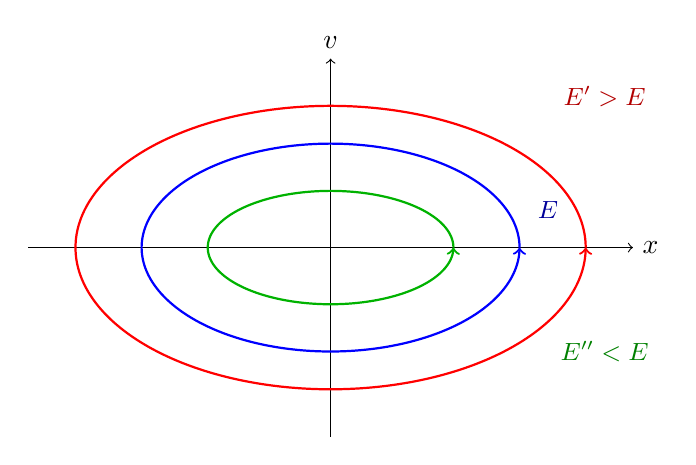
\begin{tikzpicture}[scale=1.2]
            \draw[->] (-3.2, 0) -- (3.2, 0) node[anchor=west] {$x$};
            \draw[->] (0, -2) -- (0, 2) node[anchor=south] {$v$};

            \draw[thick, green!70!black, ->] plot[smooth, domain=0:360, samples=200] 
                ({1.3*cos(\x)}, {0.6*sin(\x)});
            \draw[thick, blue, ->] plot[smooth, domain=0:360, samples=200] 
                ({2*cos(\x)}, {1.1*sin(\x)});
            \draw[thick, red, ->] plot[smooth, domain=0:360, samples=200] 
                ({2.7*cos(\x)}, {1.5*sin(\x)});

            \node[green!50!black] at (2.9, -1.1) {\small $E'' < E$};
            \node[blue!60!black] at (2.3, 0.4) {\small $E$};
            \node[red!70!black] at (2.9, 1.6) {\small $E' > E$};
        \end{tikzpicture}
        \caption{Orbita per diversi insiemi di livello $E''<E<E'$}
    \end{figure}

\end{example}

\begin{remark}
    Da $H=E$, ottengo $E-U(x)= \frac{mv^2}{2}>0\implies U(x)\leq E $.
\end{remark}
Dunque $x$ fa sempre parte dell'\textit{insieme di sottolivello} $E $ di $U \,: \left\{ x\in \mathbb{R}:U(x)\leq E  \right\}$.
\begin{definition}
    I punti in cui $v= 0 \;(U(x)= E )$ sono detti \textit{punti di inversione}.
\end{definition}
\begin{definition}
    $(x_0,0)$ è \textit{punto di equilibrio}, dato un punto di equilibrio come dato iniziale, $(x,v)\equiv(x_0,0)$ è soluzione.
\end{definition}

\begin{example}
    Oscillatore iperbolico 
    \begin{equation}
        m\ddot{x}= kx \iff \begin{cases}
            \dot{x}=v\\
            \dot{v}= \frac{k}{m}x
        \end{cases}\implies
        E = \frac{m}{2}v^2  -\frac{k}{2}x^2
    \end{equation}
    Consideriamo prima il caso in cui $E=0:$
    \begin{equation}
        mv^2  -kx^2=0 \quad \omega^2=\frac{k}{m}\implies v = \pm \omega x 
    \end{equation}
    Le soluzioni sono due linee rette che si incrociano nell'origine, ma per il teorema dell'unicità le orbite non si possono incrociare, 
    quindi in realtà sono 5 orbite separate: due semirette entranti nell'origine, due semirette uscenti dall'origine e l'origine stessa che è punto di equilibrio.
    \begin{figure}[ht]
        \centering
        \begin{tikzpicture}[scale=1.4, >=stealth]
            \draw[->, thick] (-2, 0) -- (2, 0) node[anchor=west] {$x$};
            \draw[->, thick] (0, -2) -- (0, 2) node[anchor=south] {$v$};

            \draw[thick, blue!70!black] ({1.8*cos(135)}, {1.8*sin(135)}) -- (0, 0);
            \draw[thick, blue!70!black] ({1.8*cos(315)}, {1.8*sin(315)}) -- (0, 0);

            \draw[->, thick, blue!70!black] 
                ({1.2*cos(135)}, {1.2*sin(135)}) -- ({0.75*cos(135)}, {0.75*sin(135)});
            \draw[->, thick, blue!70!black] 
                ({1.2*cos(315)}, {1.2*sin(315)}) -- ({0.75*cos(315)}, {0.75*sin(315)});

            \draw[thick, red!70!black] (0, 0) -- ({1.8*cos(45)}, {1.8*sin(45)});
            \draw[thick, red!70!black] (0, 0) -- ({1.8*cos(225)}, {1.8*sin(225)});

            \draw[->, thick, red!70!black] 
                ({0.75*cos(45)}, {0.75*sin(45)}) -- ({1.2*cos(45)}, {1.2*sin(45)});
            \draw[->, thick, red!70!black] 
                ({0.75*cos(225)}, {0.75*sin(225)}) -- ({1.2*cos(225)}, {1.2*sin(225)});

            \filldraw[violet, thick] (0, 0) circle (2.5pt);
        \end{tikzpicture}
        \caption{Le 5 orbite per $E=0$}
    \end{figure}

    Per $E \neq 0$, si ottengono delle iperboli:
    \begin{equation}
        \frac{mv^2}{2E} - \frac{kx^2}{2E} = 1
    \end{equation}
    \begin{equation}
        v^2 = \frac{2E}{m} \left( 1 + \frac{kx^2}{2E} \right) \qquad
        v = \pm \sqrt{\frac{2E}{m} \left( 1 + \frac{kx^2}{2E} \right)}
    \end{equation}
    
    \begin{figure}[ht]
        \centering
        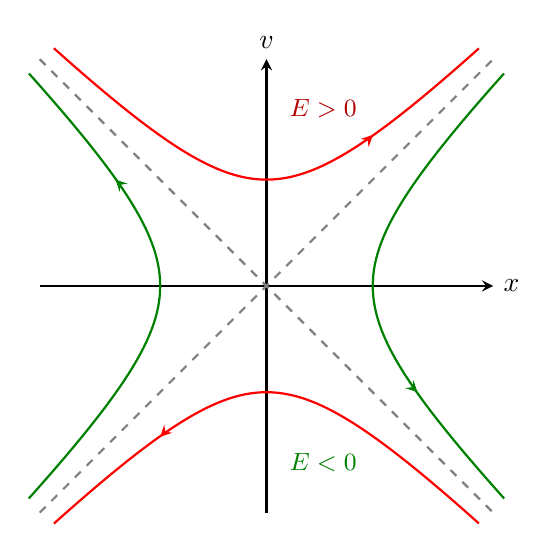
\begin{tikzpicture}[scale=0.9, >=stealth]
            % Parametri
            \def\a{1.5}  % ampiezza
            \def\omega{1} % coefficiente lineare degli asintoti

            % Assi
            \draw[->, thick] (-3.2, 0) -- (3.2, 0) node[anchor=west] {$x$};
            \draw[->, thick] (0, -3.2) -- (0, 3.2) node[anchor=south] {$v$};

            % Asintoti: v = ± omega x
            \draw[dashed, thick, gray] (-3.2,-\omega*3.2) -- (3.2,\omega*3.2);
            \draw[dashed, thick, gray] (-3.2,\omega*3.2) -- (3.2,-\omega*3.2);

            % Iperboli E>0
            \draw[thick, red]
                plot[domain=-3:3, samples=200] (\x, {sqrt(\omega^2*\x*\x + \a*\a)});
            \draw[thick, red]
                plot[domain=-3:3, samples=200] (\x, {-sqrt(\omega^2*\x*\x + \a*\a)});

            % Iperboli E<0 (x in funzione di v)
            \draw[thick, green!50!black]
                plot[domain=-3:3, samples=200, variable=\y] ({-sqrt((\y*\y + \a*\a)/\omega^2)}, \y);
            \draw[thick, green!50!black]
                plot[domain=-3:3, samples=200, variable=\y] ({sqrt((\y*\y + \a*\a)/\omega^2)}, \y);

            % Frecce direzione moto
            \draw[->, thick, red] (1.46,2.09) -- (1.5,2.13);
            \draw[->, thick, red] (-1.46,-2.09) -- (-1.5,-2.13);
            % \draw[-, thick, green!50!black] (-2.4,1) -- (-2.7,1.5);
            \draw[->, thick, green!50!black] (-2.09,1.46) -- (-2.13,1.5);

            % \draw[-, thick, green!50!black] (2.4,-1) -- (2.7,-1.5);
            \draw[->, thick, green!50!black] (2.09,-1.46) -- (2.13,-1.5);

            % Etichette energia
            \node[red!70!black] at (0.8,2.5) {\small $E>0$};
            \node[green!50!black] at (0.8,-2.5) {\small $E<0$};
        \end{tikzpicture}
        \caption{Curve di livello dell'energia per l'oscillatore iperbolico: iperboli con asintoti $v=\pm\omega x$}
    \end{figure}

\end{example}



\subsubsection{Ritratti in fase}

\begin{definition}
    Un \textit{punto critico} $x_\star$ è un punto per cui $U'(x_\star)=0$.
\end{definition}
\begin{definition}
    Se $U''(x_\star)\neq 0 $ si dice \textit{non degenere}.
\end{definition}
\begin{definition}
    Se $U''(x_\star)>0$ (minimo locale), il punto critico si dice \textit{elittico}, se $U''(x_\star)<0$ si dice \textit{iperbolico}.   
\end{definition}

Sviluppiamo di $H(x,v)$ attorno a $(x_\star,0)$
\begin{equation*}
    H(x,v) = \frac{mv^2}{2} + U(x) = U(x_\star) + U'(x_\star)(x - x_\star) + 
\end{equation*}
\begin{equation*}
    + \frac{1}{2} \left( m(v-0)^2 +U''(x_\star)(x - x_\star)^2 \right) + o(\norm{(x - x_\star, v)}^2)=
\end{equation*}
\begin{equation}
    = \frac{mv^2}{2} + \frac{1}{2} U''(x_\star)(x - x_\star)^2 + U(x_\star) + o(\norm{(x - x_\star, v)}^2)
\end{equation}

Guardiamo $H^{-1}(E)$ per $E = U(x_\star) + \Delta E$
\begin{equation}
    \Delta E = \frac{mv^2}{2} + \frac{1}{2} U''(x_\star)(x - x_\star)^2 + o(\norm{(x - x_\star, v)}^2)
\end{equation}
\begin{equation}
    o(\norm{(x - x_\star, v)}^2) \sim o(\Delta E)
\end{equation}
\begin{equation*}
    \frac{mv^2}{2} + \frac{1}{2} U''(x_\star)(x - x_\star)^2 = \Delta E + o(\Delta E)
\end{equation*}
\begin{equation}
    \Delta E \to 0\implies \;\frac{mv^2}{2} + \frac{1}{2} U''(x_\star)(x - x_\star)^2 \simeq \Delta E
\end{equation}

Se $U''(x_\star)= k>0$:
\begin{equation}
    \frac{m}{2\Delta E}v^2 + \frac{k}{2\Delta E}(x - x_\star)^2 \simeq 1
\end{equation}
Sono piccole ellissi centrate in $(x_\star, 0)$. Se invece $U''(x_\star) = -k$, otteniamo delle iperboli:
\begin{equation}
    \frac{m}{2\Delta E}v^2 - \frac{k}{2\Delta E}(x - x_\star)^2 \simeq 1
\end{equation}


Mettiamoci ora vicino a $(x_\star,0)$, ponendo $x(t)= x_\star + \xi(t)$:

\begin{equation}
    m \ddot{x} = m \ddot{\xi} = -U'(x_\star + \xi) = -U'(x_\star) - U''(x_\star)\xi + o(\norm{\xi})
\end{equation}
\begin{equation}
    \implies m \ddot{\xi} = - U''(x_\star)\xi
    \qquad U''(x_\star) > 0 \implies \ddot{\xi} = - \omega^2 \xi \qquad \omega = \sqrt{\frac{U''(x_\star)}{m}}
\end{equation}
\begin{equation}
    U''(x_\star) < 0 \implies \ddot{\xi} = \omega^2 \xi \qquad \omega = \sqrt{\frac{-U''(x_\star)}{m}}
\end{equation}
Nel secondo caso l'approsimazione si rompe, perché la particella si allontana dall'equilibrio.

\paragraph{Proprietà delle curve di livello $H(x,v)=E$}

\begin{enumerate}
    \item \textbf{Simmetria in $v$:} l'Hamiltoniana è pari in $v$, ossia $H(x,-v)=H(x,v)$. Questo implica che ogni curva di livello è simmetrica rispetto all'asse $x$.
    \begin{equation}
        v_\pm(x) = \pm \sqrt{ \frac{2}{m}(E - U(x)) }
    \end{equation}

    \item \textbf{Derivata della soluzione $v_+(x)$:} derivando rispetto a $x$, si ottiene:
    \begin{equation}
        v_+'(x) = \frac{-U'(x)}{ \sqrt{2m(E - U(x))} }
    \end{equation}
    
    \item \textbf{Punti di inversione:} sono i punti $\hat{x}$ per cui $E = U(\hat{x})$ e $U'(\hat{x}) \neq 0$ (zeri semplici). In tali punti:
    \begin{equation}
        \lim_{x \to \hat{x}^-} v_+'(x) = -\infty \qquad \lim_{x \to \hat{x}^+} v_+'(x) = +\infty
    \end{equation}
    La curva di fase in corrispondenza del punto $(\hat{x}, 0)$ ha tangente verticale. Si ha un'inversione elastica del moto: la particella si ferma e inverte la direzione.
    \item \textbf{Connessioni:} 
    \begin{itemize}
        \item \textit{Connessione omoclina:} è una curva chiusa nel piano delle fasi che parte e ritorna allo stesso punto di equilibrio iperbolico $(\bar{x}, 0)$.
         Rappresenta un'orbita di energia esattamente uguale al valore massimo locale del potenziale.
        \item \textit{Connessione eteroclina:} è una curva che collega due punti di equilibrio iperbolici distinti $(\bar{x}_1,0)$ e $(\bar{x}_2,0)$,
         corrispondenti a due massimi locali del potenziale.
    \end{itemize}
    In entrambi i casi, il tempo necessario per raggiungere l'equilibrio lungo la curva è infinito.

\end{enumerate}



\subsubsection{Periodo e tempo di volo}

\paragraph{Moti limitati e periodo}\mbox{}\\
Consideriamo orbite chiuse corrispondenti a moti periodici, limitati tra due punti di inversione $x_-(E)$ e $x_+(E)$, 
ovvero le soluzioni dell'equazione $E = U(x)$.

\begin{figure}[h]
    \centering
    \begin{tikzpicture}[scale=1.2, >=stealth]
        % Assi
        \draw[->] (-3.5, 0) -- (3.5, 0) node[below right] {$x$};
        \draw[->] (0, -2.2) -- (0, 2.2) node[left] {$v$};

        % Ellisse chiusa
        \draw[thick, blue] 
            plot[domain=0:360, samples=200] 
            ({2*cos(\x)}, {1.2*sin(\x)});

        % Frecce direzione del moto
        \draw[->, thick, blue] (0.1, 1.2) -- (0.2, 1.2);
        \draw[->, thick, blue] (-0.1, -1.2) -- (-0.2, -1.2);

        % Etichette
        \node[blue] at (1.4, 1.3) {\small $v_+(x)$};
        \node[blue] at (-1.4, -1.3) {\small $v_-(x)$};
        \node[blue] at (3, 0.5) {$\mathcal{C}_E=H^{-1}(E)$};

        \node[below] at (-2.5, 0) {\small $x_-(E)$};
        \node[below] at (2.5, 0) {\small $x_+(E)$};

        \filldraw[black] (-2, 0) circle (1pt);
        \filldraw[black] (2, 0) circle (1pt);
    \end{tikzpicture}
    \caption{Ritratto di fase per un moto periodico tra due punti di inversione $x_\pm(E)$}
\end{figure}

L'energia meccanica si conserva lungo il moto:
\begin{equation}
    H(x,v) = E = \frac{1}{2}mv^2 + U(x) \implies v_\pm(x) = \pm\sqrt{\frac{2}{m}(E - U(x))}
\end{equation}
Il periodo del moto è dato dall'integrale lungo il ciclo chiuso:
\begin{equation}
    T(E) = \oint_{\mathcal{C}_E} \dd{t} = \int_{x_-(E)}^{x_+(E)} \frac{1}{v_+(x)} \dd{x} + \int_{x_+(E)}^{x_-(E)} \frac{1}{v_-(x)} \dd{x}
\end{equation}
Per simmetria:
\begin{equation}
    T(E) = 2 \int_{x_-(E)}^{x_+(E)} \frac{1}{v_+(x)} \dd{x} = 2 \int_{x_-(E)}^{x_+(E)} \left( \frac{2}{m} (E - U(x)) \right)^{-1/2} \dd{x}
\end{equation}
\begin{figure}[h]
    \centering
    \begin{tikzpicture}[scale=1.2, >=stealth]

        % Assi
        \draw[->] (-3.5, 0) -- (3.5, 0) node[below right] {$x$};
        \draw[->] (0, -2.2) -- (0, 2.2) node[right] {$p = mv$};

        % Ellisse riempita tratteggiata
        \fill[pattern=north east lines, pattern color=blue!60]
            (2, 0) arc[start angle=0, end angle=180, x radius=2, y radius=1.2]
            arc[start angle=180, end angle=360, x radius=2, y radius=1.2];

        % Bordo ellisse
        \draw[thick, blue]
            (2, 0) arc[start angle=0, end angle=360, x radius=2, y radius=1.2];

    \end{tikzpicture}
    \caption{Orbita chiusa nel piano delle fasi $(x, p)$}
\end{figure}

Calcoliamo l'area nello spazio delle fasi $(x, p)$:
\begin{equation}
    A(E )= 2\int_{x_-(E)}^{x_+(E )}m v_+(x)\dd{x}= 2\int_{x_-(E)}^{x_+(E )} \sqrt{2m\left( E-U(x) \right)}\dd{x}
\end{equation}
\begin{proposition}
    \begin{equation}
        T(E )= \dv{A}{E}(E )    
    \end{equation}
\end{proposition}
\begin{proof}
    Sia $F(x) = \int_{\alpha}^{x} f(s)\,\dd{s}$, allora $F'(x) = f(x)$. Se $x = x(\theta)$,
    \begin{equation*}
        \dv{F}{\theta} = \dv{F}{x} \dv{x}{\theta} = f(x(\theta)) \dv{x}{\theta}
    \end{equation*}
    Analogamente, se $G(x) = \int_{x}^{\alpha} f(s)\,\dd{s}$,
    \begin{equation*}
        \dv{G}{\theta} = -f(x(\theta)) \dv{x}{\theta}
    \end{equation*}
    Dunque:
    \begin{equation*}
        \dv{A}{E} = 
        2 \int_{x_-(E)}^{x_+(E)} \frac{ m}{\sqrt{2m(E - U(x))}} \dd{x} + 
    \end{equation*}
    \begin{equation*}
        + 2 \sqrt{2m(E - U(x_+(E)))} \, \dv{x_+}{E}
        - 2 \sqrt{2m(E - U(x_-(E)))} \, \dv{x_-}{E}
    \end{equation*}
    Ma $E - U(x_+(E))$ e $E - U(x_-(E))$ sono uguali a $0$ perché punti di inversione.
    \begin{equation*}
        \dv{A}{E} = 
         \int_{x_-(E)}^{x_+(E)} \frac{ \sqrt{2m}}{\sqrt{(E - U(x))}} \dd{x}= T(E)
    \end{equation*}
\end{proof}


\paragraph{Moti illimitati e tempo di volo}\mbox{}\\
Consideriamo ora moti illimitati, in cui $U(x)\rightarrow -\infty\quad x \rightarrow\infty$.
\begin{figure}[ht]
\centering
\begin{tikzpicture}[scale=1.4, >=stealth]

    % Assi
    \draw[->] (-0.5,0) -- (4.2,0) node[below right] {$x$};
    \draw[->] (0,-1.5) -- (0,2) node[left] {$v$};

    %parabola dashed
    \draw[thick, blue,dashed, domain=-1.5:2, samples=200]
        plot({(\x)^2+0.5}, \x);

    % Parabola x(v)
    \draw[thick, blue, domain=-1:1, samples=200]
        plot({(\x)^2+0.5}, \x);

    % Area integranda sotto la curva da v=1 a v=2.3
    \begin{scope}
        %\clip (0,1) rectangle (3.5,2.3);
        \fill[pattern=north east lines, pattern color=yellow!60!black]
            ({(1)^2+0.5}, 0)
            -- plot[domain=1:1.6, samples=200]
               ({(\x)^2+0.5}, \x)
            -- ({(1.6)^2+0.5}, 0) -- cycle;
    \end{scope}

    % Contorno area
    \draw[thick, yellow!60!black, domain=1:1.6, samples=200]
        plot({(\x)^2+0.5}, \x);

    % Freccia di moto
    \draw[->, blue,thick ] (1.2, 0.85) -- (1.3, 0.9);

    % Linea tratteggiata rossa da v=1 a parabola
    \draw[red, thick,dashed] ({1^2 + 0.5}, 0) -- ({1^2 + 0.5}, 1);
    \draw[green, thick,dashed] ({1.6^2 + 0.5}, 0) -- ({1.6^2 + 0.5}, 1.6);

    \node[below,red] at (1.5, 0) {\small $\xi$};
    \node[below,green] at ({1.6^2+0.5}, 0) {\small $x$};

\end{tikzpicture}
\caption{Moto illimitato}   
\end{figure}

Calcoliamo il \textit{tempo di volo all'infinito} da un punto $x = \xi$ con $v > 0$:
\begin{equation}
    T_\xi(E) = \int_{\xi}^{+\infty} \frac{1}{v(x)}\, \dd{x} 
    = \int_{\xi}^{+\infty} \left( \frac{2}{m} (E - U(x)) \right)^{-1/2} \dd{x}
\end{equation}
Se $U(x) \to -\infty$ più velocemente di $-x^2$, allora avrò $T_\xi(E) < +\infty$,
 ovvero avrò un \textit{blow-up} a infinito in $t = T_\xi(E)$.

\begin{example}
    \begin{equation*}
        m\ddot{x}=+kx^3;\quad U(x) = -\frac{k}{4}x^4
    \end{equation*}
    Calcolare $T_\xi(E = 0)$:
    \begin{equation*}
        \frac{1}{2}mv^2 - \frac{k}{4}x^4 = E \qquad 
        v = \sqrt{\frac{2E}{m} + \frac{k}{2m}x^4} = \sqrt{\frac{4E + kx^4}{2m}}
    \end{equation*}
    \begin{equation*}
        T_\xi(E=0) = \dv{A}{E} = \dv{E} \left( \int_{x_-}^{x_+} mv \, \dd{x} \right) 
        = \dv{E} \left( \int_{x_-}^{x_+} \frac{\sqrt{m(4E - kx^4)}}{\sqrt{2}} \, \dd{x} \right)
    \end{equation*}
    \begin{equation*}
        = \left. -\int_{x_-}^{x_+} \frac{\sqrt{2k} \, x^3}{\left( m(4E - kx^4) \right)^{1/2}} \dd{x} \right|_{E=0}
        = - \int_{x_-}^{x_+} \sqrt{\frac{2}{m k}} \, x^{3/2} \dd{x}
        = \eval{\sqrt{\frac{2k}{m}} \, \frac{2}{5} x^{5/2}}_{x_-}^{x_+}
    \end{equation*}

\end{example}



\subsubsection{La prima teoria quantistica}
\begin{proposition}
    Il \textit{primo principio di quantizzazione} dice che gli unici valori consentiti per $A(E)$ sono 
    multipli interi della costante di Planck $h $
    \begin{equation}
        A(E )= n h \qquad \text{ per } n = 1,2,3,\dots
    \end{equation}
\end{proposition}
\begin{remark}
    $A(E )$ ha le dimensioni dell'azione. $[A]= [p][x]=[J][s]$
\end{remark}
E' l'azione a essere quantizzata che implica una quantizzazione dell'energia.
\begin{definition}
    Definiamo la \textit{variabile d'azione}:
    \begin{equation}
        I (E )=  \frac{A(E)}{2\pi}= \frac{nh}{2\pi}=n \hbar  ; \qquad I(E ) = \frac{1}{2\pi}\oint_{\mathcal{C}_E }p \dd{x}
    \end{equation}
\end{definition}

Invertendo $I(E )$ si ottiene $E(I )\implies E_n=E(n\hbar)$. Quando possiamo invertire? 
\begin{equation}
    \dv{A}{E}= T(E )\implies \dv{I}{E}= \frac{T}{2\pi}>0 \implies I(E ) \text{ è monotona crescente}
\end{equation}
Per cui $I(E )$ è invertibile per moti limitati.

\begin{example}
    \textbf{Oscillatore armonico}

    \begin{equation*}
        \frac{1}{2}mv^2 + \frac{k}{2}x^2 = E \quad \iff \quad \frac{p^2}{2m} + \frac{k}{2}x^2 = E
    \end{equation*}

    \begin{equation*}
        \iff \quad \frac{x^2}{\left( \frac{2E}{k} \right)} + \frac{p^2}{2mE} = 1
    \end{equation*}

    \begin{equation*}
        A(E) = \pi a b = \pi \sqrt{\frac{2E}{k}} \sqrt{2mE} = 2\pi E \sqrt{\frac{m}{k}} = \frac{2\pi E}{\omega}
    \end{equation*}

    \begin{equation*}
        \implies I(E) = \frac{E}{\omega} \quad \implies \quad E = \omega n \hbar, \quad n = 0,1,2,\dots
    \end{equation*}
\end{example}

\begin{example}
    \textbf{Keplero} \quad (per l'idrogeno, $k = e^2$)
    \begin{equation*}
        E_n = -\frac{m e^4}{2 \hbar^2 n^2}, \qquad n = 1,2,3,\dots
    \end{equation*}
\end{example}

\begin{proposition}
    Se ne ricava il \textit{secondo principio di quantizzazione}:
    \begin{equation*}
        \omega_{n,m} = \frac{E_m - E_n}{\hbar} = \frac{m e^4}{2 \hbar^3} \left( \frac{1}{n^2} - \frac{1}{m^2} \right) \qquad \text{con } m > n
    \end{equation*}
    dove $\omega_{n,m}$ è la \textit{pulsazione della radiazione emessa} dall'idrogeno al passaggio tra un livello $E_m$ e $E_n$ di energia.
\end{proposition}



\subsubsection{Problemi moti centrali conservativi}
Consideriamo ora i problemi di moto centrale conservativo con energia potenziale $U(r )$ data.

\begin{equation*}
    H = \frac{m \abs{\dot{x}}^2}{2} + U(x) = \frac{m}{2} \left( \dot{r}^2 + r^2 \dot{\theta}^2 \right) + U(r)
\end{equation*}

\begin{equation*}
    \ell = m r^2 \dot{\theta} \, \hat{z} = \ell_z \, \hat{z} \Rightarrow \dot{\theta} = \frac{\ell_z}{m r^2}
\end{equation*}

\begin{equation*}
    \Rightarrow H = \frac{m \dot{r}^2}{2} + \frac{\ell_z^2}{2 m r^2} + U(r) \equiv E
\end{equation*}

Derivando rispetto a $t$:
\begin{equation*}
    \dot{r} \left( m \ddot{r} + U'(r) - \frac{\ell_z^2}{m r^3} \right) = 0 \quad \forall\, t \in I
    \iff m\ddot{r}= \frac{l_z^2}{mr^3}-U'(r  )
\end{equation*}
Il primo pezzo rappresenta la forza centrifuga.

\begin{definition}
    Definiamo il \textit{potenziale efficace } del moto radiale:
    \begin{equation}
        U_e(r)= U(r ) + \frac{\ell_z^2}{2mr^2}
    \end{equation}
\end{definition}
Considerando il potenziale efficace torniamo a un sistema newtoniano a una dimensione:
\begin{equation}
    m\ddot{r}= - U'_e   (r )    
\end{equation}

\begin{example}
    \begin{equation}
        U(r )= -\frac{k}{r}\implies U_e(r )= -\frac{k}{r}+\frac{\ell_z^2}{2mr^2}
    \end{equation}

    \begin{figure}[h]
        \centering
        \includegraphics[width=0.6\textwidth]{images/orbitaKeplero.png}
        \caption{Energia efficace e ritratti in fase per il problema di Keplero}
    \end{figure}
    
    Sappiamo l'andamento di $U_e (r )$:
    \begin{itemize}
        \item Per $r\rightarrow \infty, \; U_e(r )\sim -\frac{k}{r}$.
        \item Per $r\rightarrow 0,\; U_e (r ) \sim \frac{\ell_z^2}{2mr^2}$.
        \item Per $r = \frac{\ell_z^2}{2mk},\;  U_e = 0$.
        \item Per $r^*= \frac{\ell_z^2}{mk},\; U'_e(r^*)=0, U_e(r^*)= U_{min}=-\frac{mk^2}{2\ell_z^2}$.
    \end{itemize}

    A seconda della sua energia $E$, l'orbita avrà diversa forma:
    \begin{itemize}
        \item Se $E<U_{min}$ non ci sarà nessuna orbita.
        \item Se $E= U_{min}$ ho un equilibrio, che corrisponde a un moto circolare uniforme: $\dot{\theta}=\frac{\ell_z^2}{mr^*}$.
        \item Se $E\in (U_{min},0)$ ho moti oscillanti radialmente.
        \item Se $E=0 $ il moto è illimitato, $\dot{r}_\pm= \sqrt{-\frac{2U_e(r )}{m }}$ che all'infinito tende a $0$, quindi il moto è una parabola.
        \item Se $E>0$ avrò moti iperbolici in cui $\dot{r}\rightarrow k \neq 0$.
    \end{itemize}

\end{example}


% Prova di grafico
% \begin{tikzpicture}[scale=1.1]
%     % Assi grafico sopra
%     \begin{scope}
%         \draw[->] (0,0) -- (6,0) node[right] {$r$};
%         \draw[->] (0,0) -- (0,4) node[above] {$U_c$};

%         \pgfmathsetmacro{\a}{5}
%         \pgfmathsetmacro{\b}{2/3*\a}

%         % Potenziale efficace (stilizzato)
%         \draw[thick, blue, domain=0.5:5.5, samples=100] 
%             plot (\x, {\a/(\x*\x+20) - \b/(\x+20)}) node[right] {};

%         % Livelli di energia (orizzontali)
%         \foreach \y/\col in {1.2/green, 1.8/red, 2.7/purple} {
%             \draw[\col, dashed] (0.5,\y) -- (5.8,\y);
%         }

%         % Linee guida verso grafico sotto
%         \foreach \x in {1.2,3.7,0.85,5.2} {
%             \draw[gray!50, very thin] (\x,0) -- ++(0,-3.5);
%         }
%     \end{scope}

%     % Grafico sotto: piano fase (r, \dot{r})
%     \begin{scope}[yshift=-5.5cm]
%         \draw[->] (0,0) -- (6,0) node[right] {$r$};
%         \draw[->] (0,-2.2) -- (0,2.2) node[above] {$\dot{r}$};

%         % Traiettoria chiusa (orbita ellittica)
%         \draw[thick, blue] plot [smooth cycle, tension=1] coordinates {(1.2,0) (1.8,1.2) (3.7,0) (1.8,-1.2)};
%         \node[blue] at (1.8,0.2) {$\circlearrowleft$};

%         % Traiettoria aperta (iperbolica)
%         \draw[thick, red, ->] plot [smooth] coordinates {(0.85,0) (1.6,1) (3,0.2) (5.2,0)};
%         \draw[thick, red, ->] plot [smooth] coordinates {(0.85,0) (1.6,-1) (3,-0.2) (5.2,0)};

%         % Traiettoria asintotica (parabolica)
%         \draw[thick, green, ->] plot [smooth] coordinates {(1.3,0) (2.3,0.9) (4,0)};
%         \draw[thick, green, ->] plot [smooth] coordinates {(1.3,0) (2.3,-0.9) (4,0)};
%     \end{scope}
% \end{tikzpicture}
\begin{example}
    Consideriamo il caso di potenziale centrale armonico:
    \begin{equation}
        U_e(r) = \frac{K r^2}{2} + \frac{\ell_z^2}{2 m r^2}
    \end{equation}
    Analizziamo i limiti:
    \begin{align*}
        r \to \infty &\implies U_e(r) \sim \frac{K r^2}{2} \\
        r \to 0 &\implies U_e(r) \sim \frac{\ell_z^2}{2 m r^2}
    \end{align*}
    Quindi $U_e(r) > 0$ per ogni $r > 0$.\\
    Il punto di minimo si trova risolvendo $U_e'(r) = 0$:
    \begin{equation*}
        U_e'(r) = K r - \frac{\ell_z^2}{m r^3} = 0 \implies r^* = \sqrt{ \frac{\ell_z^2}{mK} }
    \end{equation*}
    Il moto radiale è sempre limitato e non ci sono orbite illimitate.
\end{example}



\subsubsection{Problemi vincolati}
Il moto è soggetto a una forza, ma imponiamo anche una restrizione geometrica, 
vincoliamo il moto su una curva $\gamma$ o una superficie $\Sigma$.\\
Ovviamente, sono necessarie le reazioni vincolari per il moto sul vincolo, ma queste sono difficili da trattare
e generalmente incognite.
\begin{example}
    \textbf{Pendolo rigido} \\
    Fisso una massa $m $ su una guida rigida.
    \begin{equation}
        m\ddot{x}= -mg\hat{e }_2 +R\,;\qquad x_1^2+x_2^2 = l^2
    \end{equation}

    Passiamo a cordinate polari:
    \begin{equation*}
        \begin{cases}
            x_1 = \ell \sin \theta\\
            x_2 = -\ell \cos \theta
        \end{cases}
        \qquad
        \hat{r} = \begin{pmatrix} \sin \theta \\ -\cos \theta \end{pmatrix}, \qquad
        \hat{\theta} = \begin{pmatrix} \cos \theta \\ \sin \theta \end{pmatrix}
    \end{equation*}
    Considerando che:
    \begin{equation*}
        \ddot{x}= \left( \ddot{r}-r\dot{\theta}^2 \right)\hat{r}+ \left( 2\dot{r}\dot{\theta}+ r\ddot{\theta} \right)\hat{\theta}
        ;\quad R = R_r \hat{r}+R_\theta\hat{\theta};\quad  \hat{e}_1\cdot\hat{r}= -\cos(\theta);\quad \hat{e}_2\cdot\hat{\theta}=\sin(\theta)
    \end{equation*}
    Otteniamo:
    \begin{equation*}
        m\left( \ddot{r}-r\dot{\theta}^2 \right)\hat{r}+ m\left( 2\dot{r}\dot{\theta}+ r\ddot{\theta} \right)\hat{\theta}=
        mg\cos(\theta)\hat{r}-mg\sin(\theta)\hat{\theta}+ R_r \hat{r}+ R_\theta\hat{\theta}
    \end{equation*}
    Considerando che per il vincolo $\dot{r}=0,\ddot{r}=0$:
    \begin{equation*}
        \begin{cases}
            -mr\dot{\theta}^2=mg\cos(\theta)+ R_r\\
            mr\ddot{\theta}= -mg\sin(\theta)+ R_\theta
        \end{cases}
    \end{equation*}
    Considerando attrito nullo e quindi $R_\theta=0$, otteniamo infine il \textit{pendolo matematico}
    \begin{equation}
        \begin{cases}
            R_r  = -mg\cos(\theta)-mr\dot{\theta}^2\\
            \ddot{\theta}= -\omega^2\sin(\theta)
        \end{cases}
        \quad \text{ con } \omega = \sqrt{\frac{g}{r}}
    \end{equation}
    
    Defininendo il potenziale con una costante arbitraria $\omega^2$:
    \begin{equation}
        U(\theta)= -\omega^2\cos(\theta)+\omega^2 \implies H(\theta,\dot{\theta})= \frac{\dot{\theta}^2}{2}+ \omega^2\left( 1-\cos(\theta) \right)= E 
    \end{equation}
    Da cui possiamo ricavare le forme dell'orbite al variare di $E$:
    \begin{itemize}
        \item Per $E<0$ è impossibile e non abbiamo alcuna orbita.
        \item Per $E=0$ siamo in condizioni di equilibrio.  
        \item Per $E \in (0,2\omega^2)$ abbiamo dei moti periodici.
        \item Per $E = 2\omega^2$ abbiamo una connessione eteroclina.
        \item Per $E > \omega^2$ il pendolo continua a ruotare attorno al cerchio
    \end{itemize}

    \begin{figure}[h]
        \centering
        \includegraphics[width=0.6\textwidth]{images/orbitaPendoloRigido.png}
        \caption{Energia e ritratti in fase per il pendolo rigido}
    \end{figure}

    \paragraph{Piccole oscillazioni}
    Consideriamo il caso delle piccole oscillazioni: 
    \begin{equation*}
        \abs{\theta} \ll 1, \implies \ddot{\theta} = -\omega^2 \sin \theta \simeq -\omega^2 \theta + o(\theta^2)
    \end{equation*}
    \begin{equation*}
        H(\theta, \dot{\theta}) = \frac{\dot{\theta}^2}{2} + \frac{\omega^2 \theta^2}{2} + o(\theta^3) = E 
    \end{equation*}

    \begin{equation}
        \implies \theta(t) = \theta(0)\cos(\omega t) + \frac{\dot{\theta}(0)}{\omega} \sin(\omega t) \quad \text{ per } \abs{\theta}\ll 1
    \end{equation}

    \begin{equation}
        \implies R_r(t) \simeq m\left[ g\left( \frac{\theta(t)^2}{2} - 1 \right) - \ell \dot{\theta}^2(t) \right]
    \end{equation}

    \paragraph{Rotazioni veloci}
    Consideriamo ora il caso delle rotazioni veloci, in cui $\abs{\dot{\theta}}\gg1$:
    \begin{equation*}
        E = \frac{\dot{\theta}^2}{2} + \omega^2 (1 - \cos \theta) \simeq \frac{\dot{\theta}^2}{2}
        \implies \dot{\theta} \simeq \sqrt{2E}
    \end{equation*}
    \begin{equation}
        R_r(t) = -m \left( g \sin \theta + r \dot{\theta}^2 \right) \simeq -m r \dot{\theta}^2 = -2Emr
    \end{equation}

    \paragraph{Calcolo del Periodo}
    E' possibile calcolarci il periodo con la formula precedentemente ricavata:
    \begin{equation}
        T(E) = 2 \int_{\theta_-(E )}^{\theta_+(E)} \frac{1}{\sqrt{2\left( E - \omega^2(1 - \cos \theta) \right)}} \dd{\theta}
    \end{equation}
    Considerando la conservazione dell'energia:
    \begin{equation*}
        \dot{\theta}^2 = 2\left( E - \omega^2 (1 - \cos \theta) \right)
    \end{equation*}
    definiamo i punti di inversione $\theta_\pm(E)$ tali che $\dot{\theta} = 0$, ossia:
    \begin{equation}
        E = \omega^2(1 - \cos \theta_\pm)
    \end{equation}

    Usiamo l'identità trigonometrica $1 - \cos \theta = 2 \sin^2(\theta/2)$ per semplificare:
    \begin{equation*}
        E = \omega^2(1 - \cos \theta) = 2 \omega^2 \sin^2\left( \frac{\theta}{2} \right)
        \implies \sin^2\left( \frac{\theta}{2} \right) = \frac{E}{2\omega^2}
    \end{equation*}
    \begin{equation}
        \implies \theta_+(E) = 2 \arcsin\left( \sqrt{\frac{E}{2\omega^2}} \right)
    \end{equation}

\end{example}

\begin{example}
    \textbf{Particella sulla sfera in assenza di forze attive}\\

    La particella si muove soggetta alla reazione vincolare $R $, perciò:
    \begin{equation*}
        m \ddot{x} = R, \qquad \abs{x}^2 = r^2
    \end{equation*}

    La reazione vincolare è sempre perpendicolare alla superficie sferica, quindi è una forza centrale. 
    Di conseguenza, il momento angolare $\ell = x \times m\dot{x}$ si conserva.\\
    Il moto avviene nel piano $\ell \cdot x = 0$, che interseca la sfera in un equatore. \\
    Dalla conservazione del momento angolare segue che la velocità è costante:
    \begin{equation*}
        \abs{\ell} = m r \abs{\dot{x}} = \text{costante} \implies \abs{\dot{x}} = \text{costante}
    \end{equation*}
    Quindi la particella si muove di moto uniforme lungo una circonferenza massima della sfera.
\end{example}

